

\section{SQUISH-E Implementation}
The following sections focuses on the implementation of the elements described in the previous sections. In order to implement the algorithm, C was chosen because it allows the use of streaming technologies such as Kafka. It also allows the executable to be run at high speed because C is a compiled language, which reduces latency compared with other languages such as Python, which is an interpreted language, and Java, which runs on a Java Virtual Machine (JVM). The second advantage of this implementation choice is the use of the C language in database systems such as PostgreSQL in order to be able to implement the algorithm in MobilityDB.

In order to implement the SQUISH-E algorithm, it is necessary to follow the pseudo code and implement each component, as well as making certain implementation choices for elements that are not present in the C language. First SQUISH-E is a state-based algorithm. It does not return any output and have instead a state and update the state for each input. The output strategy chosen is like the sliding window where the last point are keep and the points are pushed into the database. 

\subsection{Algorithm 1 - SQUISH-E}

The first main loop is written as C function. The function have no return and changes the states of the variables.  This function take all the variables mentionned above it has some types and struct that will be described down. 

\begin{lstlisting}[float=h,language=C, % Spécifie le langage du code
caption={SQUISH-E}, % Légende du listing
label=lst:squish_c, % Étiquette pour référencer le listing
numbers=left,
numberstyle=\tiny\color{gray},
stepnumber=1,
frame=single,
breaklines=true,
postbreak=\mbox{\textcolor{red}{$\hookrightarrow$}\space},
showstringspaces=false
]

void
iteration_simplification_sqe(void *p_i , void *p_j ,
size_t *beta,const double lambda,int i,
Dict *succ,Dict *pred,
PDict  *p,struct PriorityQueue *Q,
bool syncdist,interpType interp ,bool hasz ,uint32_t minpts)
{
	if( i * lambda >= *beta)
	{
		*beta += 1;
	}
	set_priority_queue(p_i,INF,Q);
	set_priority_dict(p_i,0,p);
	if(i >= 1)
	{
		set_point_dict(p_i,p_j,pred);
		set_point_dict(p_j,p_i,succ);
		adjust_priority(p_j,Q,pred,succ,p, syncdist, interp , hasz );
	}
	size_t size = size_queue(Q);
	if(size - *beta == 0 ){
		reduce(Q,pred,succ,p,syncdist, interp , hasz );
	}
}
\end{lstlisting}


This algorithm \ref{lst:squish_c} follow the pseudo code of SQUISH-E it called the set function of the priority queue and the set function of the point map and priority map that will be describe in the section about implementation of variable. Then the reduce function and adjust priority is called in order to reduce if the size meet the treshold and the adjustment for each point that has a predecessor and a successor in order to know the error that it will produce by removing the corresponding point.

\subsection{Algorithm 2 - Reduce}
Then we have the main block of SQUISH-E which is the reduce part.

\begin{lstlisting}[language=C, % Spécifie le langage du code
caption={reduce}, % Légende du listing
label=lst:reduce_c, % Étiquette pour référencer le listing
numbers=left,
numberstyle=\tiny\color{gray},
stepnumber=1,
frame=single,
breaklines=true,
postbreak=\mbox{\textcolor{red}{$\hookrightarrow$}\space},
showstringspaces=false,
float,
floatplacement=H
]

void
reduce(struct PriorityQueue *Q,Dict *pred,Dict *succ,PDict  *p,
bool syncdist,interpType interp ,bool hasz )
{
	struct PriorityQueueElem *entry = remove_min(Q);
	size_t size_before = size_queue(Q);
	
	void * p_j = entry->point;
	double priority = entry->priority;
	
	void * p_i = get_point_dict(p_j,pred);
	void * p_k = get_point_dict(p_j,succ);
	
	double pr_i = get_priority_dict(p_i,p); if(priority > pr_i){ pr_i = priority; }
	double pr_k = get_priority_dict(p_k,p); if(priority > pr_k){ pr_k = priority; }
	
	set_priority_dict(p_k, pr_k ,p);
	set_priority_dict(p_i, pr_i ,p);
	
	set_point_dict(p_i,p_k,succ);
	set_point_dict(p_k,p_i,pred);
	set_point_dict(p_k,p_i,pred);
	
	adjust_priority(p_k ,Q,pred,succ,p,syncdist, interp ,hasz );
	adjust_priority(p_i ,Q,pred,succ,p,syncdist, interp ,hasz );
	
	
	//Delete pointer
	free(entry);
	destroy_elem_PriorityDict(p_j,p);
	destroy_elem_PointDict(p_j,succ);
	destroy_elem_PointDict(p_j,pred);
}

\end{lstlisting}

This algorithm \ref{lst:reduce_c} describe the reduction method as mentioned above remove the lowest priority points from the queue and it update the neighbors. Because we use C langage we free memory of the useless data. Each call is represented by a function in order to simplify implementation and reduce it to pieces of code to be written for each particular variable. This choice of implementation also makes it possible to change the structure. 

\subsection{Algorithm 3 - Adjust Priority} 

\begin{lstlisting}[language=C, % Spécifie le langage du code
caption={adjust\_priority}, % Légende du listing
label=lst:adjust_c, % Étiquette pour référencer le listing
numbers=left,
numberstyle=\tiny\color{gray},
stepnumber=1,
frame=single,
breaklines=true,
postbreak=\mbox{\textcolor{red}{$\hookrightarrow$}\space},
showstringspaces=false,
float,
floatplacement=H
]

void
adjust_priority(void *p_i,struct PriorityQueue *Q, Dict *pred,Dict *succ,PDict  *p,
bool syncdist,interpType interp ,bool hasz )
{

	void * p_h = get_point_dict(p_i,pred);
	void * p_k = get_point_dict(p_i,succ);
	if( p_h != NULL &&  p_k != NULL )
	{
		if(syncdist)
		{
			double priority = get_priority_dict(p_i,p) + SED(p_h,p_i,p_k, interp , hasz );
			set_priority_queue(p_i,priority,Q);
		}
	}
}

\end{lstlisting}
 

This algorithm \ref{lst:adjust_c} is what differentiates SQUISH from SQUISH-E: when a point is removed, the surrounding points are updated and their priority changed, so we only recover the neighbours and calculate the new priority on the basis of the old error present in the dictionary and the calculation of the synchronised Euclidean distance. 


\section{Variables Implementation}
In this section we'll discuss how the variables have been implemented and how effective they are, followed by a discussion of the performance and complexity achieved.

\subsection{Map}
In this section we will focus on the implementation of the map

\begin{lstlisting}[float=h,language=C, % Spécifie le langage du code
caption={Map C implementation}, % Légende du listing
label=lst:map_c, % Étiquette pour référencer le listing
numbers=left,
numberstyle=\tiny\color{gray},
stepnumber=1,
frame=single,
breaklines=true,
postbreak=\mbox{\textcolor{red}{$\hookrightarrow$}\space},
showstringspaces=false
]

#include <search.h>


typedef struct PriorityDict
{
void * key;
double priority;
} PriorityDict;


typedef struct PointDict
{
void *key;
void *value;
} PointDict;


typedef void* Dict;
typedef void* PDict;

\end{lstlisting}
 

This structure \ref{lst:map_c} is a Map that link a point to a corresponding value like priority or another point. We just need to define a struct with two values the key and the value. The typedef void* is using for the GNU Library to avoid using void** and add more clarity to the code.

\paragraph{Method}

\begin{lstlisting}[float=h,language=C, % Spécifie le langage du code
caption={Point Map Methods}, % Légende du listing
label=lst:pmap_c, % Étiquette pour référencer le listing
numbers=left,
numberstyle=\tiny\color{gray},
stepnumber=1,
frame=single,
breaklines=true,
postbreak=\mbox{\textcolor{red}{$\hookrightarrow$}\space},
showstringspaces=false
]

void *
get_point_dict(void *p_i,Dict *dict)
{
	PointDict find;
	find.key = p_i;
	void * result = tfind(&find, dict, compar);
	if(result){
		result = (*(PointDict**)result)->value;
	}
	return result;
}

void
set_point_dict(void * p_i,void * p_j,Dict *dict)
{
	PointDict *find = malloc(sizeof(PointDict));
	find->key = p_i;
	find->value = p_j;
	void * result = tfind(find, dict, compar);
	if(result){
		(*(PointDict**)result)->value = p_j;
	}
	else{
		tsearch(find, dict, compar); /* insert */
	}
}

void destroy_elem_PointDict(void * p_i,Dict *dict)
{
	PointDict find;
	find.key = p_i;
	void * r = tfind(&find, dict, compar);
	if(r)
	{
		PointDict * to_free = (*(PointDict**)r);
		tdelete(&find,dict,compar);
		free(to_free);
	}
}

\end{lstlisting} 

Here \ref{lst:pmap_c} we use function of GNU C Library that implement a binary tree. It has the property to have for each operation a maximal complexity of $O(log(n))$ The two mapping use the same implementation in reality it would be a good idea to resolve this duplication case using a template or thing that can resolve it but the C language limit the capability.

\paragraph{Discussion}
As mentioned in the previous sub section the map use GNU C Library binary tree structure to perform search and set. Those algorithm have a complexity of $O(log(n))$ as mentioned before and it has the property to be have a dynamic allocation of memory.

\subsection{PriorityQueue}

\begin{lstlisting}[float=h,language=C, % Spécifie le langage du code
caption={PriorityQueue}, % Légende du listing
label=lst:prqueue_c, % Étiquette pour référencer le listing
numbers=left,
numberstyle=\tiny\color{gray},
stepnumber=1,
frame=single,
breaklines=true,
postbreak=\mbox{\textcolor{red}{$\hookrightarrow$}\space},
showstringspaces=false
]

typedef struct PriorityQueueElem
{
	void * point;
	double priority;
	int index; //reference his own index
} PriorityQueueElem;

typedef void* IDict;

typedef struct PriorityQueue
{
	PriorityQueueElem **arr;
	IDict dict;
	size_t size;
	size_t capacity;
} PriorityQueue;

\end{lstlisting} 

This structure \ref{lst:prqueue_c} implements the function of a priority queue using the structure of a min heap. It has as value PriorityQueueElem which have the point and the corresponding priority and a reference to this index in the heap. The main structure is using an array of pointer of PriorityQueueElem as long as an index map, a int that represent the number of points in the queue and lastly the numbers points allocated.

\paragraph{Method}

Once the skeleton of the algorithm has been implemented. To finish the implementation, the methods of the variables described can be implemented. 

\begin{lstlisting}[float=h,language=C, % Spécifie le langage du code
	caption={PriorityQueue Remove Min}, % Légende du listing
	label=lst:prqueueMethodR_c, % Étiquette pour référencer le listing
	numbers=left,
	numberstyle=\tiny\color{gray},
	stepnumber=1,
	frame=single,
	breaklines=true,
	postbreak=\mbox{\textcolor{red}{$\hookrightarrow$}\space},
	showstringspaces=false
]
	
PriorityQueueElem *remove_min(PriorityQueue *Q)
{
	PriorityQueueElem *result = NULL;
	if (Q->size != 0) {
		result = Q->arr[0];
		// Replace the deleted node with the last node
		Q->arr[0] = Q->arr[Q->size - 1];
		Q->arr[Q->size - 1] = NULL;
		if(Q->arr[0]){
			Q->arr[0]->index = 0;
		}
		
		// Decrement the size of heap
		Q->size--;
		
		tdelete(result,&Q->dict,compar_index);
		// Call minheapify_top_down for 0th index
		// to maintain the heap property
		minHeapify(Q, 0);
	}
	return result;
}
\end{lstlisting}

So, in order to remove the point with the minimum result, the following procedure \ref{lst:prqueueMethodR_c} is used: we check the number of elements and retrieve the first element. The insertion methods ensure that the first element is always the one with the minimum result. Then we take the last element and remove it and place it at the beginning of the queue and balance the tree to keep the smallest element at index 0. Then remove the index from the dictionary. 


\begin{lstlisting}[float=h,language=C, % Spécifie le langage du code
caption={PriorityQueue Set Elem}, % Légende du listing
label=lst:prqueueMethodSet_c, % Étiquette pour référencer le listing
numbers=left,
numberstyle=\tiny\color{gray},
stepnumber=1,
frame=single,
breaklines=true,
postbreak=\mbox{\textcolor{red}{$\hookrightarrow$}\space},
showstringspaces=false
]

void
set_priority_queue(void *p_i,double priority ,PriorityQueue *Q)
{
	struct PriorityQueueElem * insert = replace_elem(p_i,priority,Q);
	if(insert == NULL){
		insert = malloc(sizeof(struct PriorityQueueElem));
		insert->point = p_i;
		insert->priority = priority;
		insert->index = -1;
		tsearch(insert, &Q->dict, compar_index); /* insert */
	}
	if(insert->index == -1){
		push(insert,Q);
	}
}


struct PriorityQueueElem *
replace_elem(void *p_i,double priority ,PriorityQueue *Q)
{
	PriorityQueueElem *elem = get_elem(p_i,&Q->dict);
	if(elem ){
		if(Q->size > elem->index && elem->index != -1){
			Q->arr[elem->index]->priority = priority;
			insertHelper(Q, elem->index);
			minHeapify(Q, elem->index);
		}
	}
	return elem;
}
	
void
push(PriorityQueueElem * insert,PriorityQueue *Q)
{
	Q->size++;
	if(Q->size > Q->capacity){
		Q->arr = realloc(Q->arr, Q->size * sizeof(PriorityQueueElem*));
	}
	Q->arr[Q->size-1] = insert;
	Q->arr[Q->size-1]->index = Q->size-1;
	insertHelper(Q, Q->size-1);
}

\end{lstlisting}

From other implementation this one \ref{lst:prqueueMethodSet_c} has the property to have at most a complexity of $O(log(n))$ the choice of a min heap to implement the priorityqueue fullfill the complexity limitation that we see in the design phase. The min heap is structure has a structure of a tree like we see in Figure \ref{fig:min_heap} and has the property that each tree and sub tree has the property that the parent nodes is always lesser than the child nodes. The min heap implementation is inspired from this website \cite{GfG_2023}. 


\begin{figure}[!h]
\centering
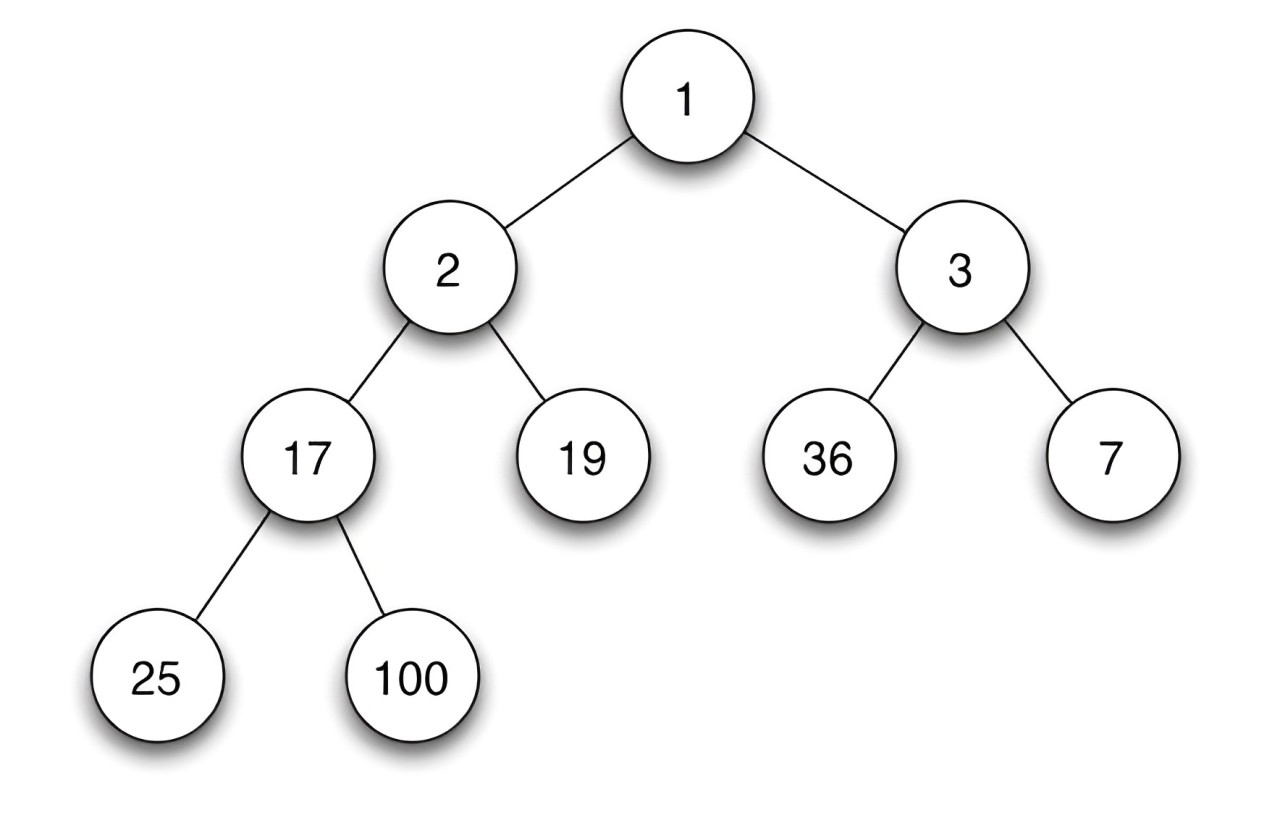
\includegraphics[width=1\linewidth]{figures/tree.jpeg}
\caption{Min Heap Structure}
\label{fig:min_heap}
\end{figure}


\paragraph{Discussion}

The idea here is to use the min heap structure to obtain in a complexity of maximum $O(log(n))$  the point with the lowest priority. In the side we use a index map in order to replace point in the heap in an efficient way. Due to the fact that the design include the set of an element when it is already in the array. This structure has the advantage to benefit from static memory. The set works using the mapping to see if the point is already present in the map. If it is we replace it in the heap by changing his priority and apply a check with his ancestor then his descendant. If the point is not present we add a value at the end of the heap and check and update their ancestor to satisfy the condition of a min heap. So at the end the two operations needed for the algorithm reach a complexity of $O(log(n))$

\section{PostgreSQL Implementation}

In this section we describe how the algorithm is implemented into the MobilityDB sql functions.
\subsection{SQL Code}
As the implementation is in C, the implementation of the sql code \ref{lst:squish_sql} is only a reference to the C function.\\

\begin{minipage}{\linewidth}
\begin{lstlisting}[
language=SQL, % Setting the language for SQL
caption={SQUISHE SQL Code}, % Caption for the listing
label=lst:squish_sql, % Label for referencing the listing
basicstyle=\ttfamily\small, % Basic style
keywordstyle=\color{blue}\ttfamily, % Style for keywords
stringstyle=\color{red}\ttfamily, % Style for strings
commentstyle=\color{green}\ttfamily, % Style for comments
numbers=left, % Line numbers on the left
numberstyle=\tiny\color{gray}, % Style for line numbers
stepnumber=1, % Line numbers step
frame=single,
breaklines=true, % Automatic line breaking
postbreak=\mbox{\textcolor{red}{$\hookrightarrow$}\space}, % Arrow for line breaks
showstringspaces=false % Don't show special spaces within strings
]
CREATE FUNCTION SquishESimplify(tfloat, float, boolean DEFAULT TRUE)
RETURNS tfloat
AS 'MODULE_PATHNAME', 'Temporal_simplify_sqe'
LANGUAGE C IMMUTABLE STRICT PARALLEL SAFE;
CREATE FUNCTION SquishESimplify(tgeompoint, float, boolean DEFAULT TRUE)
RETURNS tgeompoint
AS 'MODULE_PATHNAME', 'Temporal_simplify_sqe'
LANGUAGE C IMMUTABLE STRICT PARALLEL SAFE;
\end{lstlisting}
\end{minipage}

\subsection{Example}
This section show some examples of usages of the pgsql function describe in \ref{lst:squish_sql}. This allowed to use the algorithm in an offline settings using request.\\


\begin{minipage}{\linewidth}
\begin{lstlisting}[
language=SQL, % Setting the language for SQL
caption={Example SQL Code}, % Caption for the listing
label=lst:example_sql, % Label for referencing the listing
basicstyle=\ttfamily\small, % Basic style
keywordstyle=\color{blue}\ttfamily, % Style for keywords
stringstyle=\color{red}\ttfamily, % Style for strings
commentstyle=\color{green}\ttfamily, % Style for comments
numbers=left, % Line numbers on the left
numberstyle=\tiny\color{gray}, % Style for line numbers
stepnumber=1, % Line numbers step
frame=single,
breaklines=true, % Automatic line breaking
postbreak=\mbox{\textcolor{red}{$\hookrightarrow$}\space}, % Arrow for line breaks
showstringspaces=false % Don't show special spaces within strings
]

SELECT SquishESimplify(tfloat '[1@2000-01-01, 2@2000-01-02, 3@2000-01-04,
4@2000-01-05]', '1 day');
-- [1@2000-01-01, 3@2000-01-04]

SELECT asText(SquishESimplify(tgeompoint '[Point(1 1 1)@2000-01-01,
Point(2 2 2)@2000-01-02, Point(3 3 3)@2000-01-04, Point(5 5 5)@2000-01-05)', 0.5));
-- [POINT Z (1 1 1)@2000-01-01, POINT Z (3 3 3)@2000-01-04,POINT Z (5 5 5)@2000-01-05)

\end{lstlisting}
\end{minipage}
